\section{String Diagrams}
\label{sec:string-diagrams}
In this section, we illustrate the axioms of concatenation using string diagrams.

This diagram shows \cref{ax:cons-snoc-symmetry} about the symmetry of definitions of $\pureterm$ and $\binconcatterm$.
    \begin{center}
        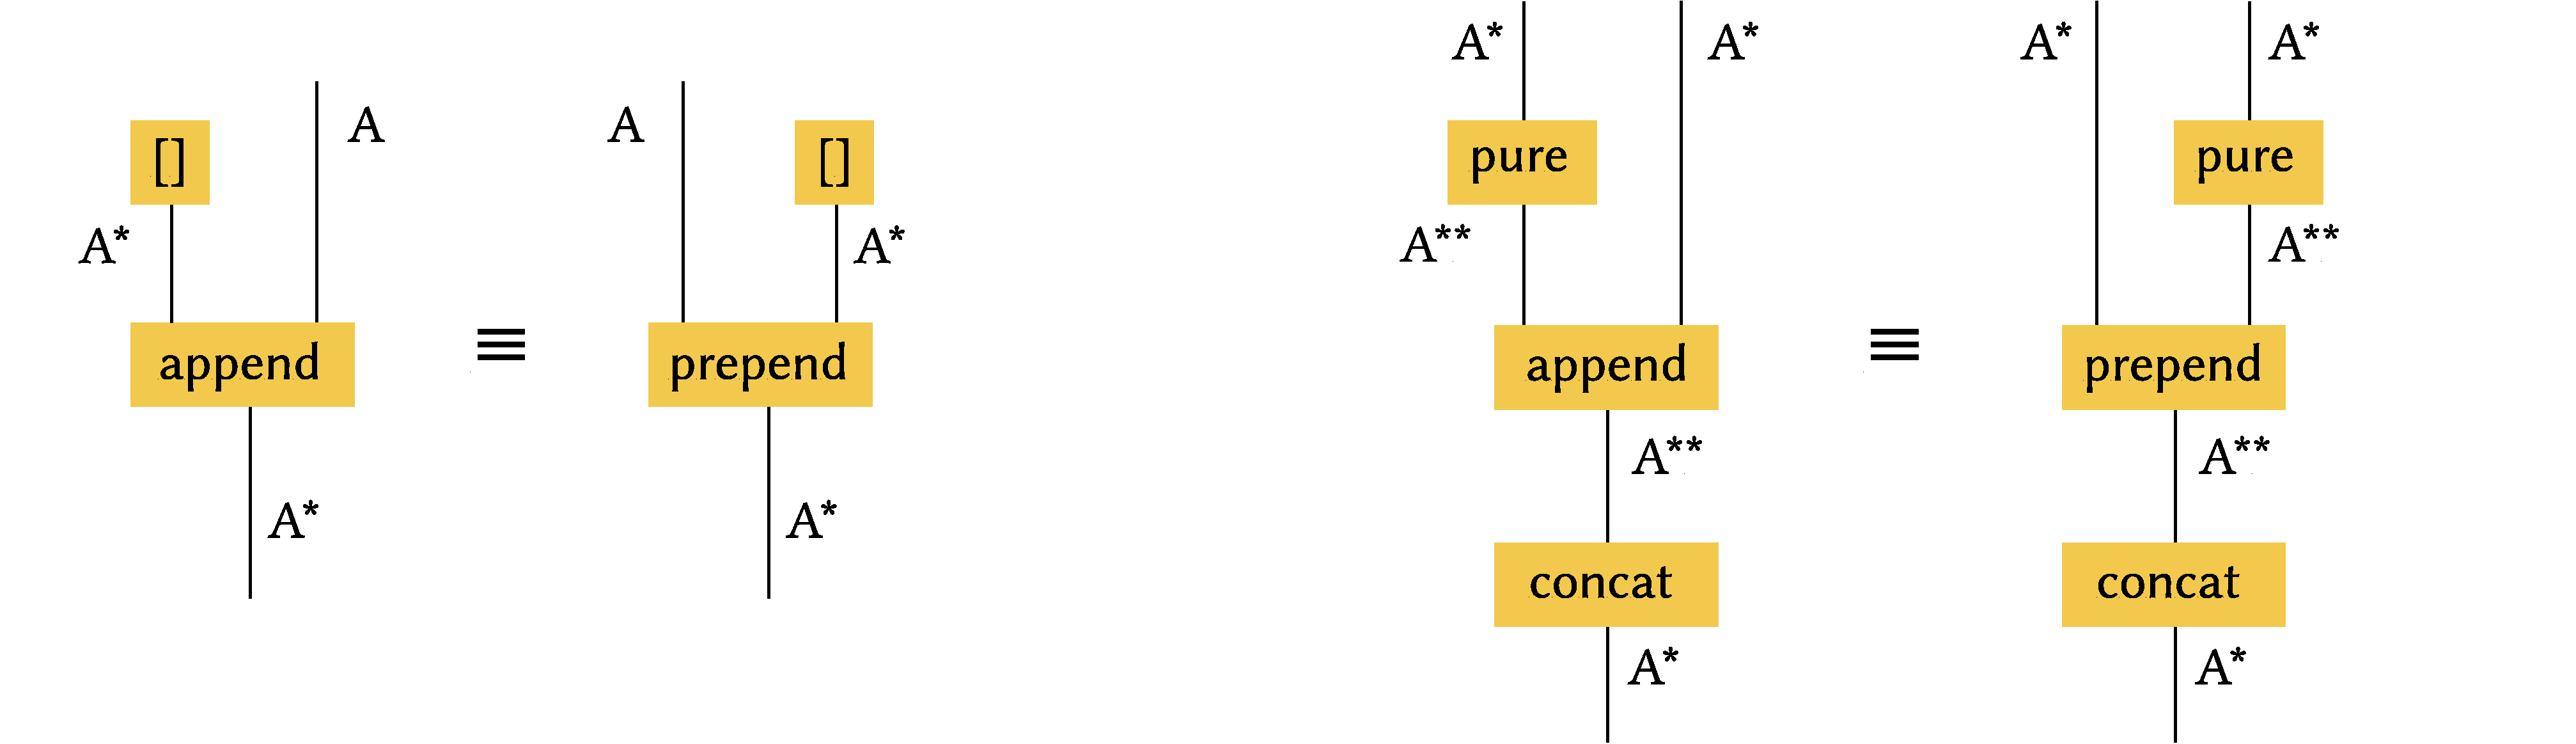
\includegraphics[page=1,scale=0.2]{B-string-diagrams/equational-theory-rational}
    \end{center}

This diagram shows     \cref{ax:concatenation-monoid}: $A^*$ is a monoid with respect to $\binconcatterm$ and $[]$.
    \begin{center}
        \includegraphics[page=2,scale=0.2]{B-string-diagrams/equational-theory-rational}
    \end{center}

This diagram shows      \cref{ax:concat-monoid-homomorphism}: $\concatterm$ is a monoid homomorphism from $A^{**}$ to $A^*$.
    \begin{center}
        \includegraphics[page=3,scale=0.2]{B-string-diagrams/equational-theory-rational}
    \end{center}

This diagram shows     \cref{ax:from-monoid-to-inductive}: $\prependterm$ and $\appendterm$ defined in terms of $\pureterm$ and $\binconcatterm$.
    \begin{center}
        \includegraphics[page=4,scale=0.2]{B-string-diagrams/equational-theory-rational}
    \end{center}

